\section{Data Capture}
\label{sec:datacapture}

\subsection{Hardware}
\label{sec:hardware}

We utilized the capture setup proposed by Kider et al. to capture data needed to train and predict sky radiance distribution curves for the sun/skydome\cite{kider_framework_2014}. This novel hardware system captured spectral, spatial, and temporal information, including radiance, HDR fisheye imagery, and total irradiance, simultaneously for various sky conditions. Fig.~\ref{fig:hardwarejtk}(left) shows the capture setup on the roof of a building. The system includes a custom-built spectral radiance measurement scanner to measure the directional spectral radiance, using an ASD FieldSpec Pro spectroradiometer to capture field measures of the solar spectrum between 350-2500nm (Fig.~\ref{fig:hardwarejtk}(a)). The system used a commercial digital camera to capture HDR hemispherical imagery of the sky, using a Canon 5D with a Sigma 8mm circular fish-eye lens, following a similar scanning technique to Stumpfel et al.\cite{Stumpfel:2004}. This approach utilized 8 exposures to span a range of 17 stops of the sun and sky to capture a wide dynamic range (Fig.~\ref{fig:hardwarejtk}(b)). Lastly, the system used an Apogee pyranometer to measure a total irradiance value of the sun/sky (Fig.~\ref{fig:hardwarejtk}(c)).

\begin{figure}[hbtp]
\begin{center}
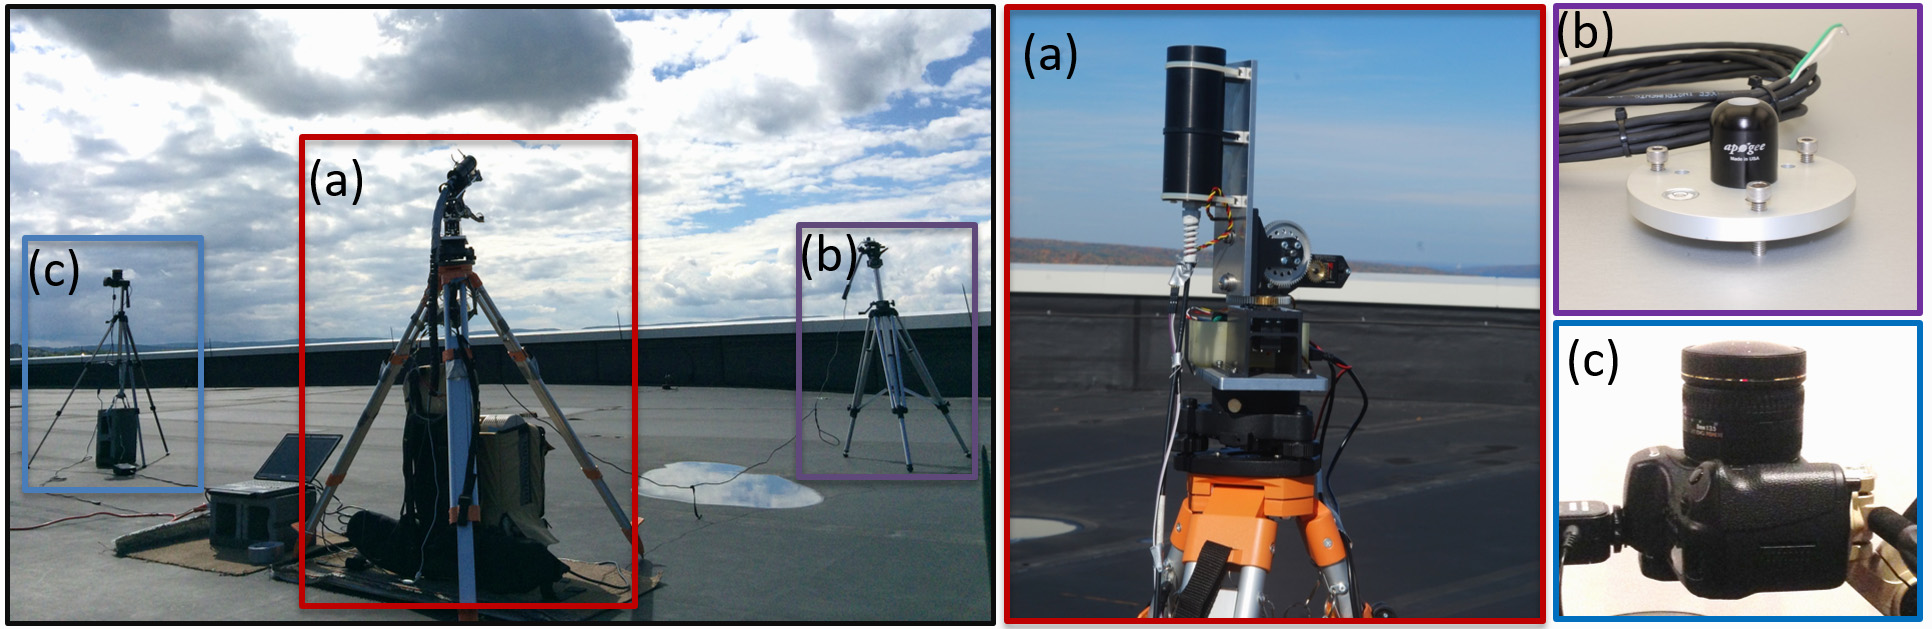
\includegraphics[width=0.98\textwidth]{img/hardware.jpg}
\end{center}\vspace{-2mm}
\caption[hardwarejtk] {\label{fig:hardwarejtk} Hardware setup of different capture devices from Kider et al.\cite{kider_framework_2014} used to capture data for this project. (a) A custom-built radiance scanner measures spectral radiance between 350-2500nm using a $1\degree$ fore-optic lens; (b) Apogee pyranometer, which measures the irradiance of the entire sun/sky; (c) Canon 5D commercial camera with Sigma 8mm circular fish-eye lens captures HDR imagery of the sun and skydome.}
\end{figure}

\subsection{Measurements}
\label{sec:measurements}

\begin{figure}[hbtp]
\begin{center}
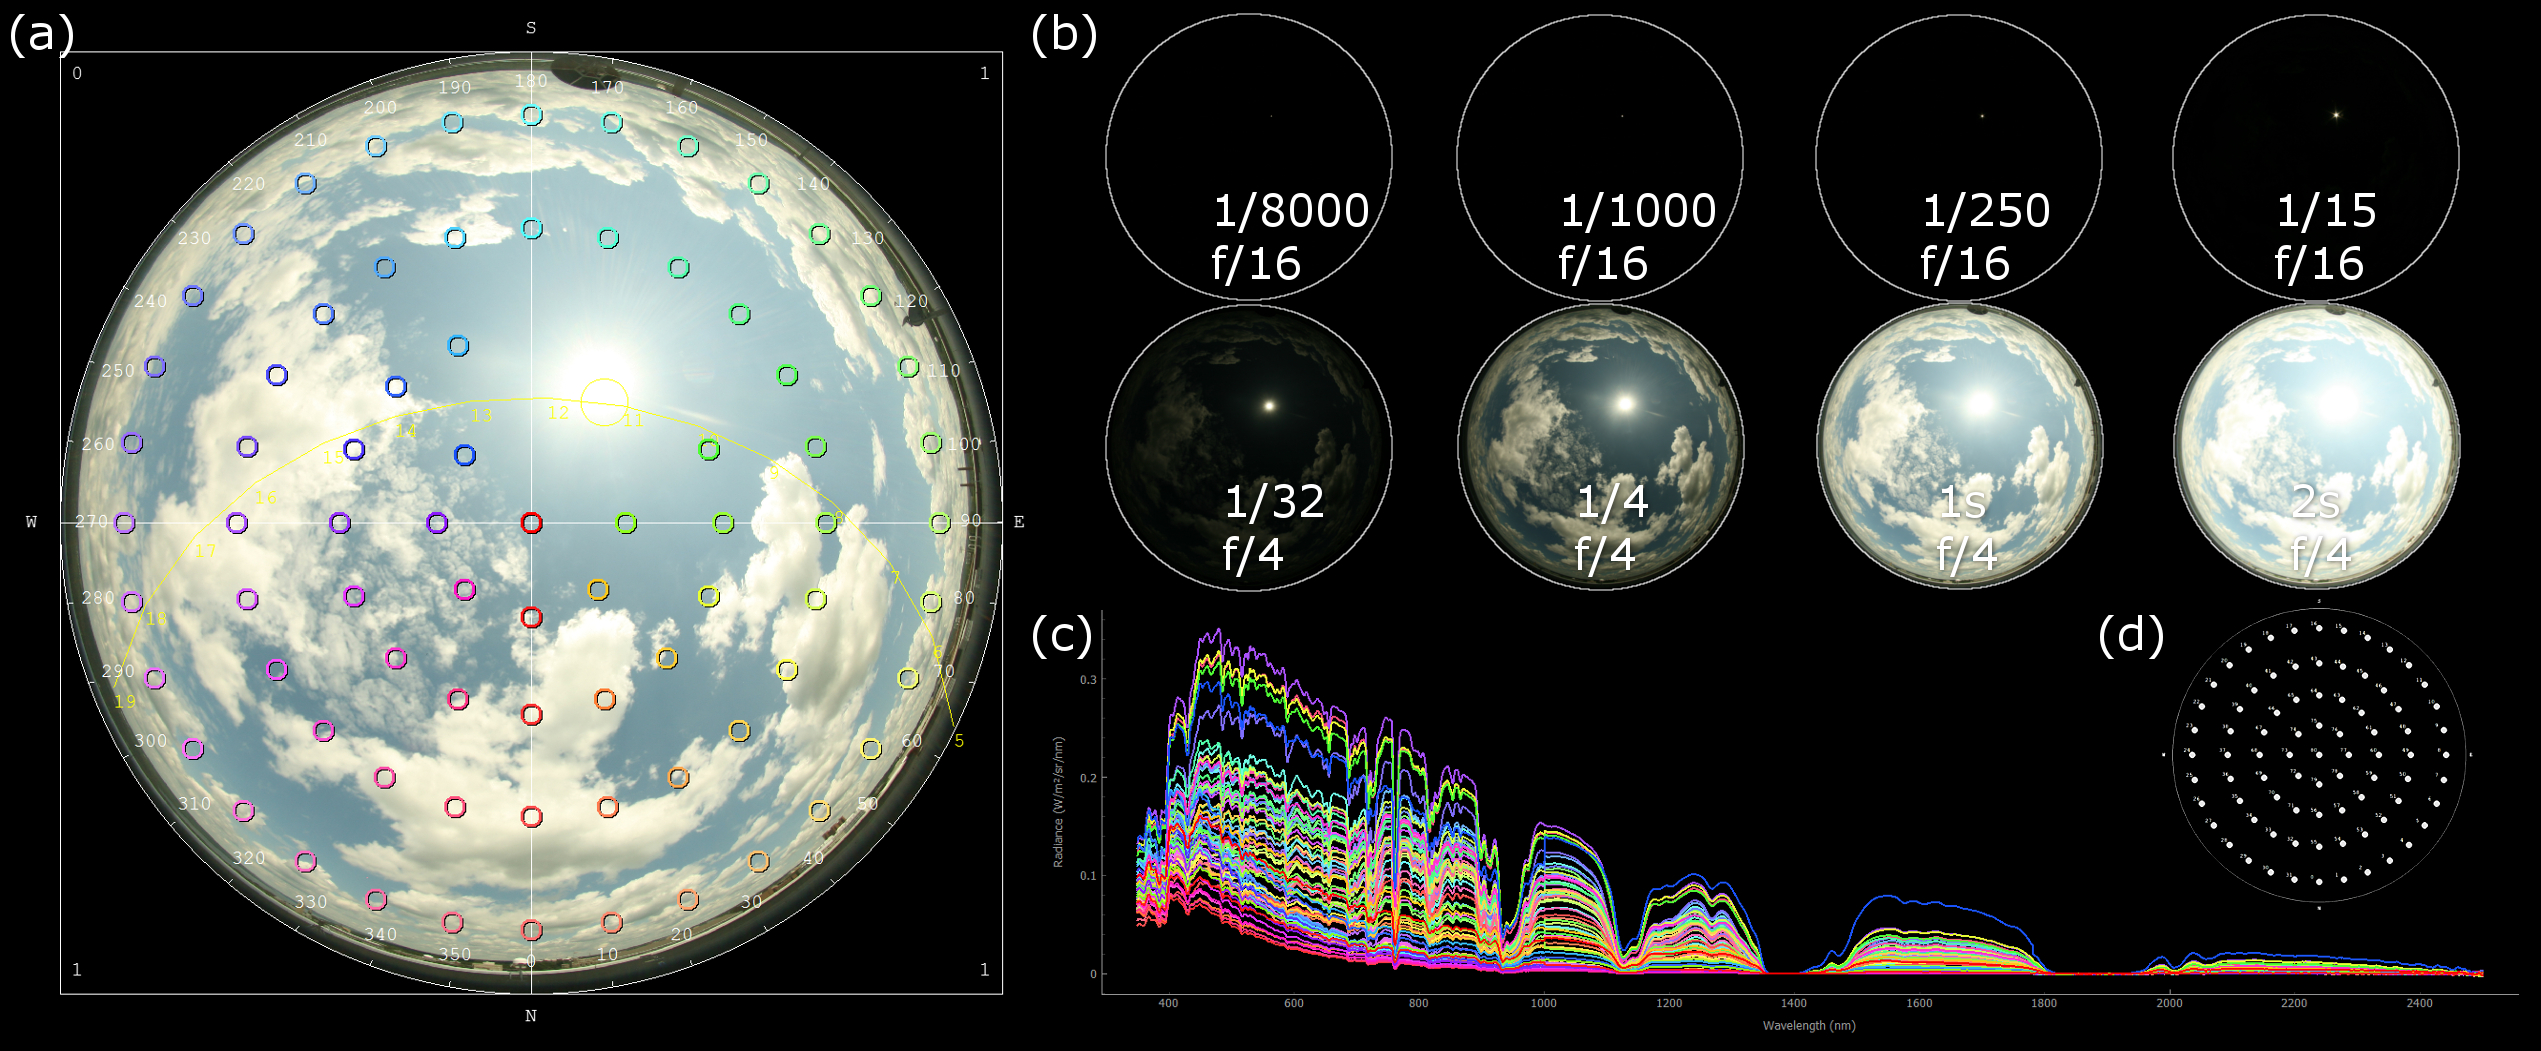
\includegraphics[width=1.0\textwidth]{img/data_measurements.jpg}
\end{center}
\caption{\label{fig:measurements}Each data capture includes: (a) a hemispherical photo of the sky, at (b) 8 separate exposures (HDR), and (c) corresponding sky radiance curves, measured at 81 points in the sky with sampling pattern (d). Applying $20\degree$ circumsolar avoidance, only 76 of the 81 points of measurement are shown in (a).}
\end{figure}

% \begin{figure}[H]
% \begin{minipage}{0.45\linewidth}
% \centering
% \includegraphics[width=1.0\textwidth]{img/data_samples.png}
% \end{minipage}%
% \begin{minipage}{0.53\linewidth}
% \centering
% \includegraphics[width=1.0\textwidth]{img/data_exposures.png} \\
% \includegraphics[width=1.0\textwidth]{img/data_radiance.png}
% \end{minipage}
% \caption{\label{fig:measurements}Each data capture includes: (a) hemispherical photo of the sky, (b) with 8 separate exposures (HDR), and (c) corresponding sky radiance distributions measured at 81 points in concentric rings. Applying $20\degree$ circumsolar avoidance, only 76 of the 81 points of measurement are shown in (a). }
% \end{figure}

% \begin{figure}[H]
% \begin{center}
% \begin{tabular}[b]
% \includegraphics[width=0.4\textwidth]{img/data_samples.png}
% \end{tabular}
% \begin{tabular}[b]
% \includegraphics[width=0.6\textwidth]{img/data_radiance.png} \\
% \includegraphics[width=0.6\textwidth]{img/data_radiance.png}
% \end{tabular}
% \end{center}
% \caption{\label{fig:measurements}Types of data we measured...}
% \end{figure}

Throughout this work, hemispherical sky coordinates are specified as $(azimuth, ~altitude)$, where $altitude$ is the complement of $zenith$ (90\degree - $zenith$), and $azimuth$ is a horizontal angle increasing eastward from north. Note that our sky photos have north and south inverted due to hardware orientation during capture.

Sky photos were captured at a resolution of 4368x2912 pixels in both JPG and CR2 (Canon Raw) formats in an sRGB color space (one of the highest pixel resolutions for custom-built sky viewers to date). As shown in Fig.~\ref{fig:measurements}, 8 separate photos were taken in sequence with exposures $1/8000s$, $1/1000s$, $1/250s$, $1/15s$, $1/32s$, $1/4s$, $1s$, $2s$, and $f$-stops $f/16$ and $f/4$. Radiance was measured in $W/m^2/sr/nm$ for 81 evenly distributed $1\degree$ solid angles across the sky. Our spectroradiometer produced a single uniform curve from 350-2500nm, containing VIS (380-760nm), VNIR (380-1400nm), and SWIR (1000-2500nm) spectra.

We used the National Renewable Energy Laboratory's (NREL) Solar Position Algorithm (SPA)\cite{reda_spa} to accurately compute the sun's hemispherical coordinates and path. Some have claimed NREL's SPA algorithm to be too computationally expensive for real-time applications, recommending the SG2 algorithm instead,\textsuperscript{\citenum{blanc_sg2},\citenum{chauvin_modelling_2015}} but we found it to be fast and reliable.

\subsection{Data}
\label{sec:data}

All data for this work was captured between 2012-2013 from the rooftop of Frank Rhodes Hall, Cornell University, Ithaca, New York, United States, decimal degrees: (42.443441, -76.481638). Although we measured data well over 1000 times over 41 days throughout the year, with multiple projects in mind, our vetted subset for this work consists of 453 captures over 16 days at differing times of day, covering many  different solar angles, all four seasons, and in general a wide variety of atmospheric conditions. These measurements are listed in Table \ref{tab:ourdata}, and hosted online for the public's benefit.\footnote{\url{https://spectralskylight.github.io/RadianceEstimationData}}

As noted in Sec.~\ref{sec:measurements}, each data capture consists of 8 sky photos (of varying exposure) and 81 radiance curves. A single training/testing sample consists of information extracted from one of these sky photos along with its corresponding directional radiance measurement. Of our 453 total captures intended to be used for this work, 22996 of the 36693 $(453\times81)$ samples were finally used for training and cross-validation testing. At least 3000+ samples were culled by circumsolar avoidance to avoid the possibility of oversaturation of direct sunlight on our samples, a common approach in many sky models,\cite{chauvin_modelling_2015} and important for our RGB-to-curve mapping. We used the same $20\degree$ region as Tohsing et al.\cite{tohsing_validation_2014} Note the effects of stray light are drastically reduced at an angle of $20\degree$.\cite{saito_estimation_2016} Many of the remaining samples culled from our final datasets are due in some part to careful examination of the measurements. This was done with an open-source, cross platform application we developed to load and visualize the measurements.\footnote{\url{https://spectralskylight.github.io/SkyDataViewer}} Although a supervised process, it allowed us to quickly navigate the abundance of data to identify dropped, locked, missing, obscured, or oversaturated measurements.

Regarding sky cover, although automatic/procedural assessment is certainly possible,\cite{yamashita_cloud, tohsing_validation_2014, saito_cloud, li_cloud, cazorla_development_2008, arking_cloudcover} we manually assessed our images to ensure accuracy during machine learning. Efficient algorithms can and should be used to automatically assess sky cover during real-time application of this work, for determining which trained model to use. Like Lee,\cite{lee_jr_measuring_2008} we use the standard categorization of sky conditions provided by the US National Oceanic and Atmospheric Administration (NOAA).\cite{noaa_fmh1chpt9_2017} We focus on the following three: clear (CLR), scattered (SCT), and overcast (OVC), where CLR and OVC represent 0 and 8 oktas of cloud cover, respectively.\cite{noaa_fmh1chpt9_2017} In this work, SCT is used to describe skies with any cloud coverage between 1-7 oktas. We ignore the distinction of few (FEW) and broken (BKN) skies to simplify the number of machine learning models that might be used in a practical setting. In theory, our models can be trained on any sky condition.

\begin{figure} [hbtp]
\begin{center}
\begin{tabular}{c}
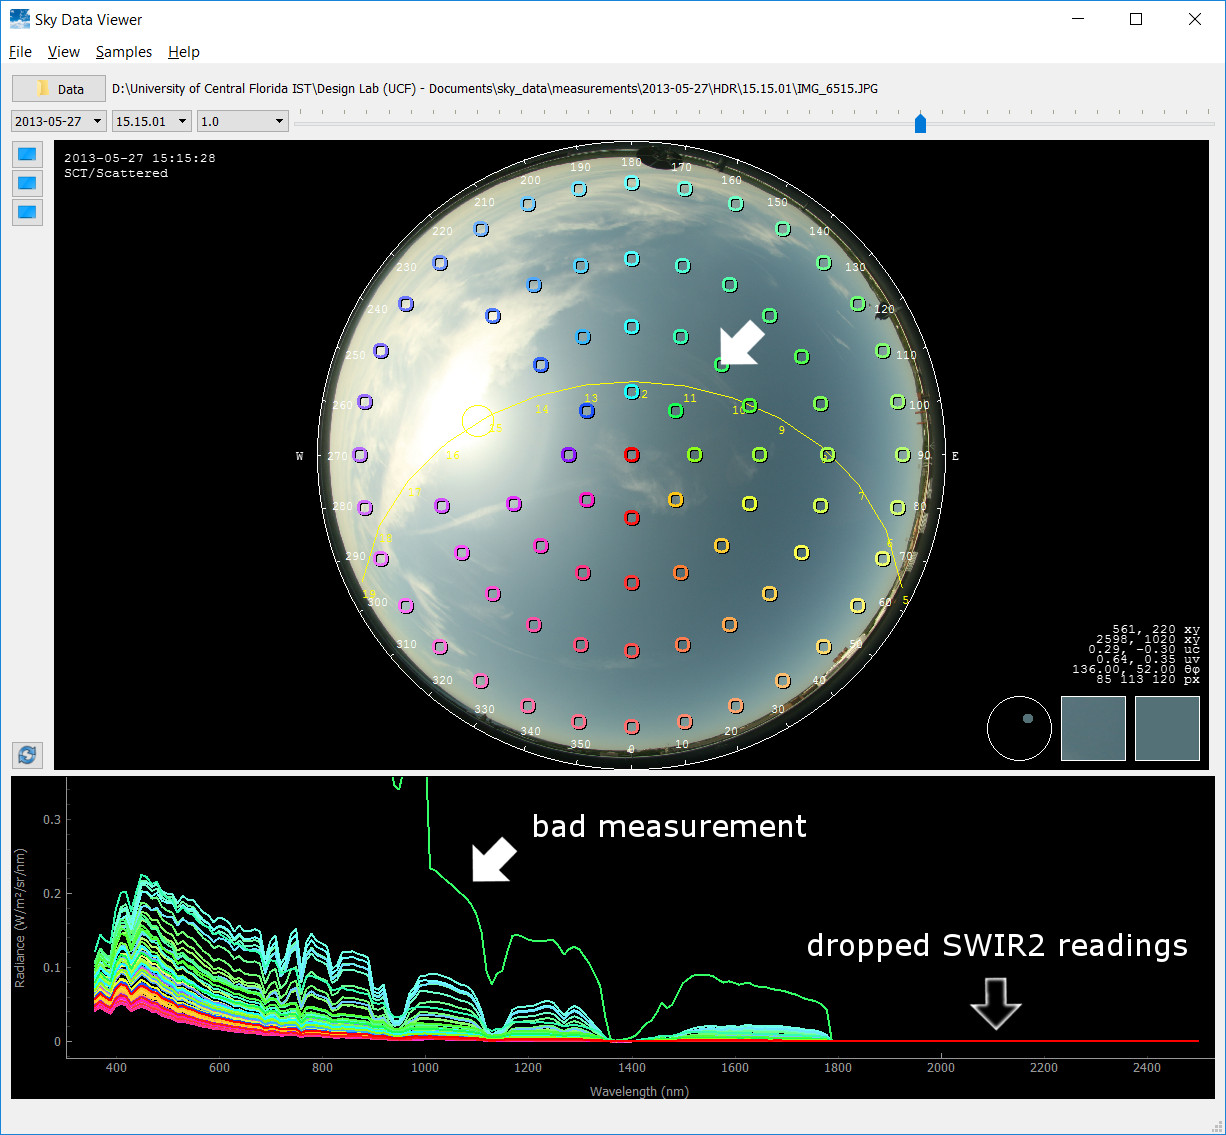
\includegraphics[width=0.485\textwidth]{img/data_badmissing.jpg}
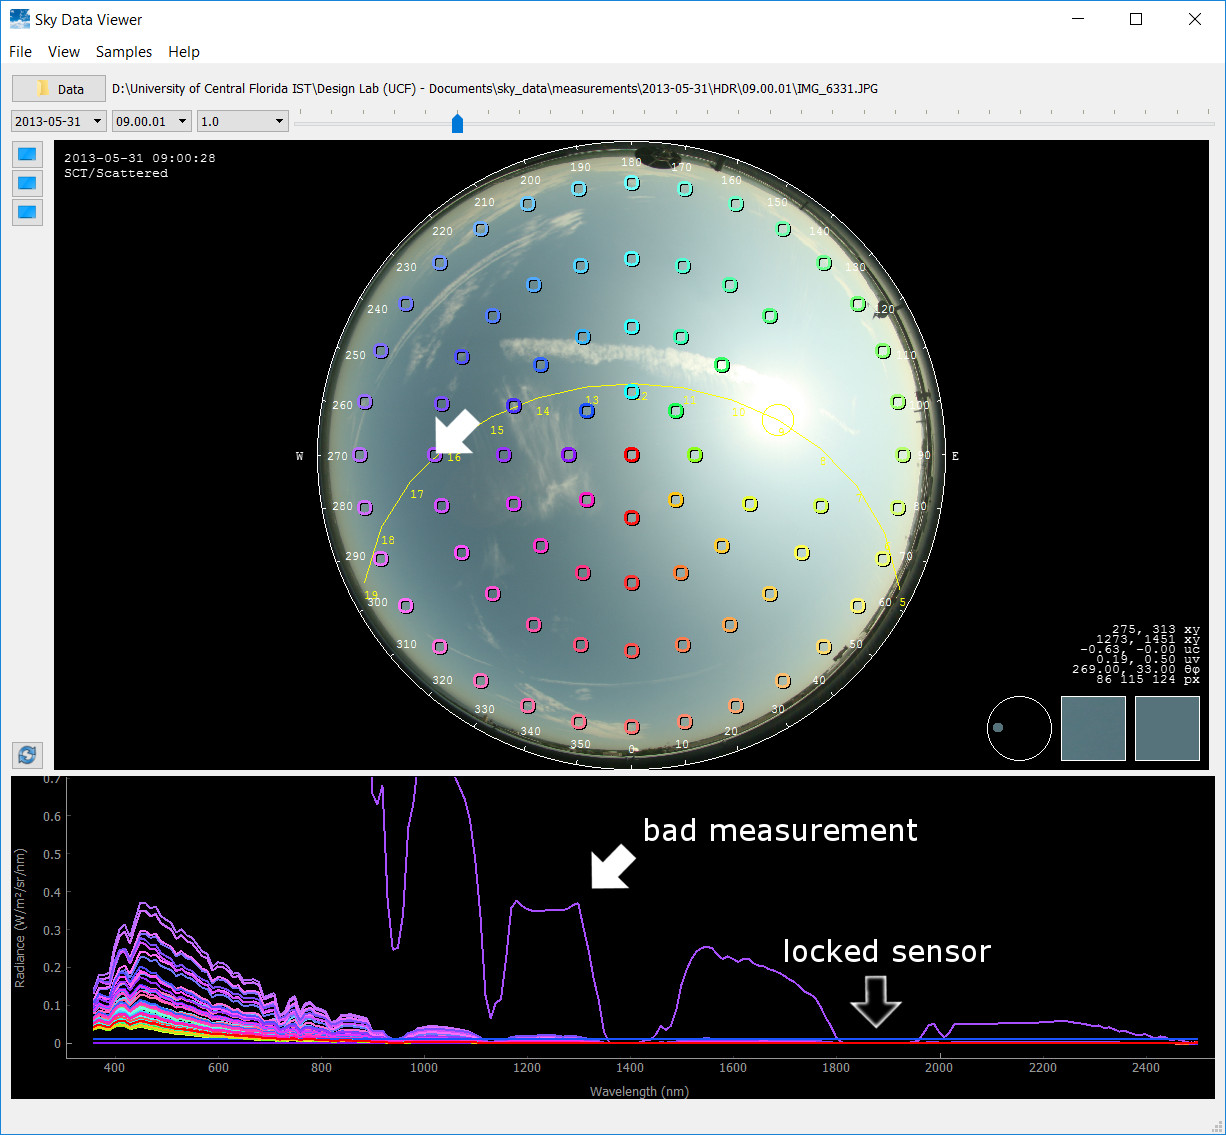
\includegraphics[width=0.485\textwidth]{img/data_badlocked.jpg}
\end{tabular}
\end{center}
\caption[skydataviewer] { \label{fig:skydataviewer} Capturing data \textit{in the wild} for machine learning algorithms is a difficult process. Errors in data capture can vastly affect ML training. Therefore, we developed a SkyDataViewer to help identify data anomalies.}
\end{figure}

\begin{table}[hbtp]
\caption{List of observed data captures, which include correlated HDR images and radiance distributions.}
\label{tab:ourdata}
\centering      
\begin{tabular}{ll*{3}{c}}
    \\
    \toprule
    \multicolumn{1}{c}{Date} & \multicolumn{1}{c}{Time} & Captures & Samples & Sky Cover(s) \\
    \midrule
    \rule[-1ex]{0pt}{3.5ex}  11/06/2012 & 12:26 - 16:21 & 41 & 3321 & SCT  \\
    \rule[-1ex]{0pt}{3.5ex}  11/15/2012 & 11:15 - 16:26 & 56 & 4536 & CLR, SCT  \\
    \rule[-1ex]{0pt}{3.5ex}  04/13/2013 & 09:55 - 10:01 & 2 & 162 & OVC  \\
    \rule[-1ex]{0pt}{3.5ex}  04/14/2013 & 10:42 - 18:36 & 46 & 3726 & SCT, OVC  \\
    \rule[-1ex]{0pt}{3.5ex}  04/15/2013 & 07:38 - 08:03 & 8 & 648 & SCT, OVC  \\
    \rule[-1ex]{0pt}{3.5ex}  05/12/2013 & 10:30 - 13:45 & 14 & 1134 & SCT, OVC  \\
    \rule[-1ex]{0pt}{3.5ex}  05/26/2013 & 10:30 - 17:30 & 29 & 2349 & CLR, SCT  \\
    \rule[-1ex]{0pt}{3.5ex}  05/27/2013 & 09:30 - 18:30 & 37 & 2997 & CLR, SCT  \\
    \rule[-1ex]{0pt}{3.5ex}  05/30/2013 & 09:30 - 12:45 & 14 & 1134 & SCT  \\
    \rule[-1ex]{0pt}{3.5ex}  05/31/2013 & 09:00 - 15:00 & 25 & 2025 & SCT  \\
    \rule[-1ex]{0pt}{3.5ex}  06/15/2013 & 07:45 - 18:30 & 44 & 3564 & CLR, SCT  \\
    \rule[-1ex]{0pt}{3.5ex}  07/26/2013 & 11:00 - 14:45 & 16 & 1296 & CLR, SCT  \\
    \rule[-1ex]{0pt}{3.5ex}  07/29/2013 & 09:00 - 14:00 & 21 & 1701 & SCT, OVC  \\
    \rule[-1ex]{0pt}{3.5ex}  08/30/2013 & 09:15 - 14:00 & 18 & 1458 & SCT, OVC  \\
    \rule[-1ex]{0pt}{3.5ex}  09/24/2013 & 06:49 - 18:09 & 38 & 3078 & CLR  \\
    \rule[-1ex]{0pt}{3.5ex}  09/26/2013 & 08:30 - 15:40 & 44 & 3564 & SCT  \\
    \midrule
    \multicolumn{1}{c}{16 Days} & & 453 & 36693 &  \\
    \bottomrule
\end{tabular}
\end{table}
